%%%%%%%%%%%%%%%%%%%%%%%%%%%%%%%%%%%%%
%                                   %
% Compile with XeLaTeX and biber    %
%                                   %
% Questions or comments:            %
%                                   %
% joshua dot mcneill at uga dot edu %
%                                   %
%%%%%%%%%%%%%%%%%%%%%%%%%%%%%%%%%%%%%

\documentclass{beamer}
  % Read in standard preamble (cosmetic stuff)
  %%%%%%%%%%%%%%%%%%%%%%%%%%%%%%%%%%%%%%%%%%%%%%%%%%%%%%%%%%%%%%%%
% This is a standard preamble used in for all slide documents. %
% It basically contains cosmetic settings.                     %
%                                                              %
% Joshua McNeill                                               %
% joshua dot mcneill at uga dot edu                            %
%%%%%%%%%%%%%%%%%%%%%%%%%%%%%%%%%%%%%%%%%%%%%%%%%%%%%%%%%%%%%%%%

% Beamer settings
% \usetheme{Berkeley}
\usetheme{CambridgeUS}
% \usecolortheme{dove}
% \usecolortheme{rose}
\usecolortheme{seagull}
\usefonttheme{professionalfonts}
\usefonttheme{serif}
\setbeamertemplate{bibliography item}{}

% Packages and settings
\usepackage{fontspec}
  \setmainfont{Charis SIL}
\usepackage{hyperref}
  \hypersetup{colorlinks=true,
              allcolors=blue}
\usepackage{graphicx}
  \graphicspath{{../../figures/}}
\usepackage[normalem]{ulem}
\usepackage{enumerate}

% Document information
\author{M. McNeill}
\title[FREN2001]{Français 2001}
\institute{\url{joshua.mcneill@uga.edu}}
\date{}

%% Custom commands
% Lexical items
\newcommand{\lexi}[1]{\textit{#1}}
% Gloss
\newcommand{\gloss}[1]{`#1'}
\newcommand{\tinygloss}[1]{{\tiny`#1'}}
% Orthographic representations
\newcommand{\orth}[1]{$\langle$#1$\rangle$}
% Utterances (pragmatics)
\newcommand{\uttr}[1]{`#1'}
% Sentences (pragmatics)
\newcommand{\sent}[1]{\textit{#1}}
% Base dir for definitions
\newcommand{\defs}{../definitions}


  % Packages and settings

  % Document information
  \subtitle[Température et narration]{La température et la narration}

\begin{document}
  % Read in the standard intro slides (title page and table of contents)
  \begin{frame}
    \titlepage
    \tiny{Office: % Basically a variable for office hours location
Gilbert 121\\
          Office hours: % Basically a variable for office hours
 lundi, mercredi, vendredi 10:10--11:10
}
  \end{frame}

  \begin{frame}{Pourquoi pas?}
    Pourquoi est-ce que ces étudiants ne sont pas venus en classe?
    \begin{columns}
      \column{0.5\textwidth}
        \small
        \begin{enumerate}
          \item Ben: sa grand-mère / téléphoner
          \item<2->[$\to$] Sa grand-mère lui a téléphoné.
          \item<3-> Adrien: il / être malade
          \item<4->[$\to$] Il était malade.
          \item<5-> Guillaume: son chien / manger ses devoirs
          \item<6->[$\to$] Son chien a mangé ses devoirs.
          \item<7-> Claire: elle / avoir un accident
          \item<8->[$\to$] Elle a eu un accident.
          \item<9-> Grégory: il / faire 25 degrés
          \item<10->[$\to$] Il faisait 25 degrés.
        \end{enumerate}
      \column{0.5\textwidth}
        \begin{minipage}[0.6\textheight]{\linewidth}
          \begin{center}
            \only<1-2>{
              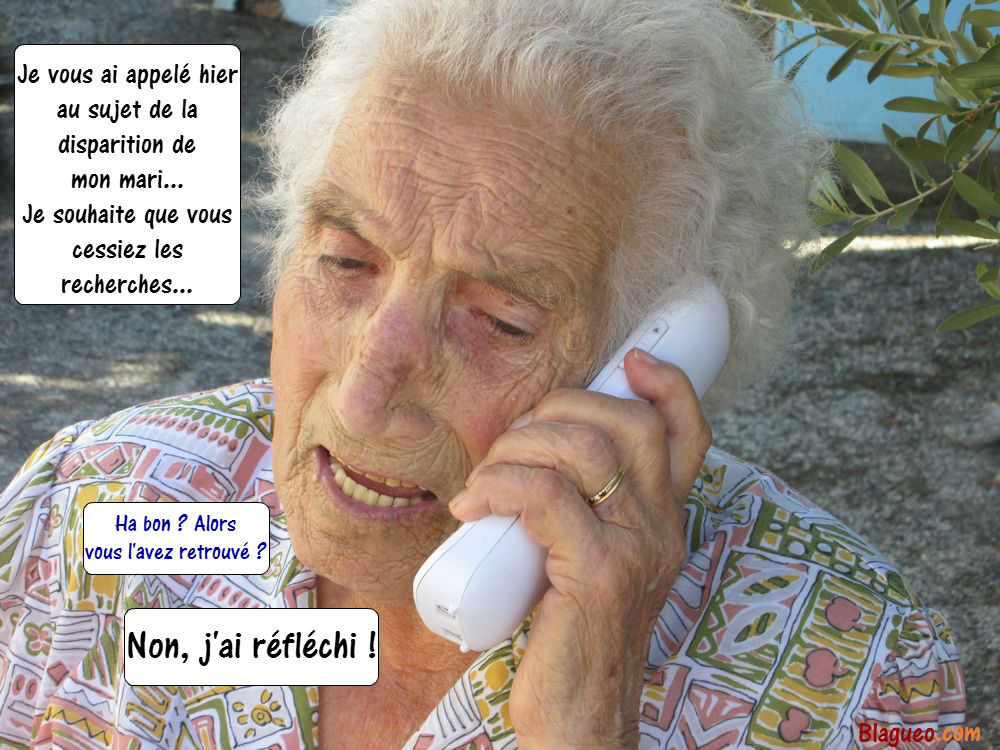
\includegraphics[scale=0.16]{téléphoner.jpg}
            }
            \only<3-4>{
              
\includegraphics[scale=0.32]{malade.jpg}
            }
            \only<5-6>{
              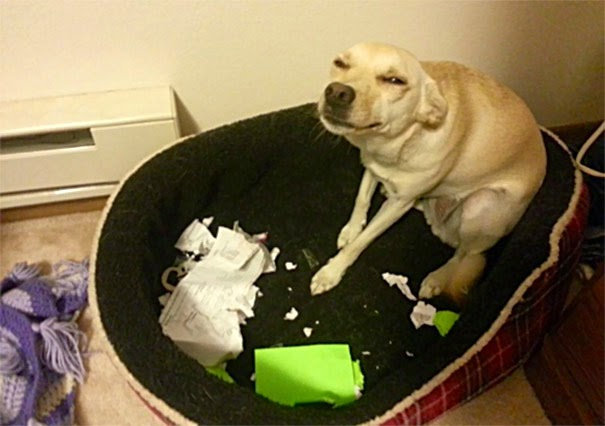
\includegraphics[scale=0.27]{chien_devoirs.jpg}
            }
            \only<7-8>{
              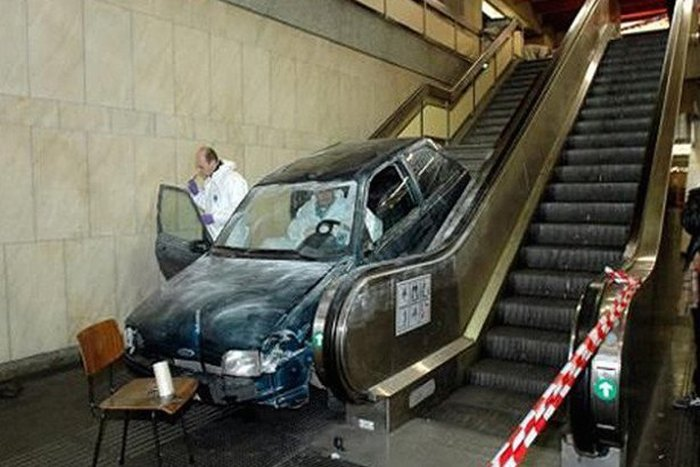
\includegraphics[scale=0.24]{accident.jpg}
            }
            \only<9-10>{
              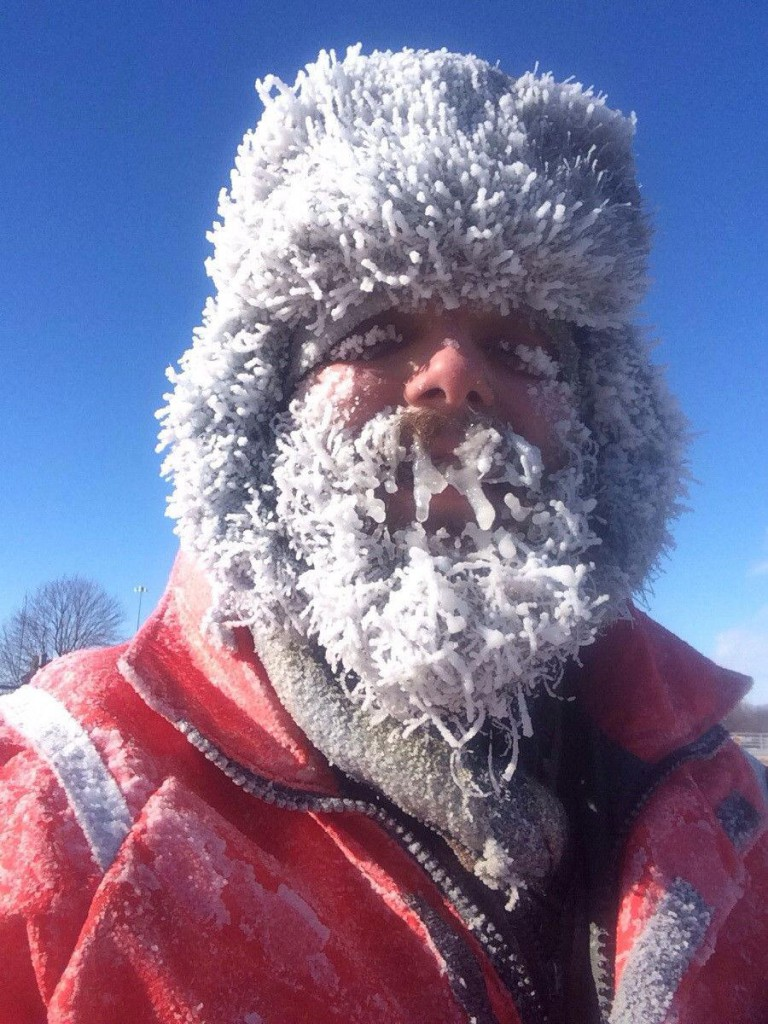
\includegraphics[scale=0.17]{froid.jpg}
            }
          \end{center}
        \end{minipage}
    \end{columns}
  \end{frame}

  \begin{frame}{}
    \begin{center}
      \Large Quiz
    \end{center}
  \end{frame}

  \begin{frame}{Qu'est-ce qu'ils ont fait?}
    \small
    En groupes de 3 ou 4, imaginez une histoire pour un de ces dessins.
    Utilisez l'imparfait et le passé composé.
    Écrivez l'histoire sur un papier.
    \begin{columns}[t]
      \column{0.5\textwidth}
        \begin{enumerate}
          \item \includegraphics[scale=0.38]{scène1.png}
          \item \includegraphics[scale=0.38]{scène2.png}
        \end{enumerate}
      \column{0.5\textwidth}
        \begin{enumerate}
          \setcounter{enumi}{2}
          \item \includegraphics[scale=0.38]{scène3.png}
          \item \includegraphics[scale=0.38]{scène4.png}
        \end{enumerate}
    \end{columns}
  \end{frame}

  \begin{frame}{}
    \begin{center}
      \Large Questions?
    \end{center}
  \end{frame}
\end{document}
